% Very simple template for lab reports. Most common packages are already included.
% !TeX spellcheck = en_US
\documentclass[a4paper, 11pt]{article}
\usepackage[utf8]{inputenc} % Change according your file encoding
\usepackage{graphicx}
\usepackage{url}

%opening
\title{Report 1: Rudy - A rudimentary web server}
\author{Bernardo González Riede}
\date{\today{}}

\begin{document}

\maketitle

\section{Introduction}


As mentioned in the assignment paper, the purpose of this assignment is to learn:
\textit{ \begin{itemize}
\item the procedures for using a socket API
\item the structure of a server process
\item the HTTP protocol
\end{itemize}}
The knowledge which is acquired through these concepts mark the fundaments of communication through a network.
\\
Sockets are the base for all communications towards external processes.
Sometimes they are even used for communicaion between processes residing on the same machine.
\\
HTTP is a widely used protocol for web servers.

\section{Main problems and solutions}

One problem encountered was how to simulate different scenarios and participants.
Since the exercise is only a small web server, all test could have been realized on the same machine (running Windows 10).
Still, the thirst for performing real world test with physical networks and GNU/Linux servers was far too attractive.
Therefore the test involved three participants:

\begin{table}[h]
\centering
\begin{tabular}{lcccc}
Name            & CPU       & RAM   & Location  & OS\\\hline
clientLocal     & 4-core    & 4GB   & KTH Kista & Windows 10\\\hline
server          & 1-core    & 512MB & Frankfurt & Ubuntu-server 16.04\\\hline
clientRemote    & 1-core    & 512MB & Frankfurt & Ubuntu-server 16.04\\\hline
\end{tabular}
\caption{Information about the participants}
\label{tab:participants}
\end{table}
The two Ubuntu machines were hosted on Digital Ocean's Datacenter in Frankfurt, Germany.
It's a virtualized datacenter, hence the incomplete description about their hardware.

\section{Evaluation}

5 scenarios were used to test the web server.
\begin{itemize}
    \item A: Rudy \& test executed on clientLocal.
    \item B: Rudy \& test executed on server.
    \item C: Rudy on server \& test on clientLocal.
    \item D: Rudy on server \& test on clientRemote.
    \item E: Rudy on server while test was executed on both clients simulatenously.
\end{itemize}

The following table results from doing 100 request to the server.
An artificial delay of 40ms was introduced in a second run to simulate file handling.
\begin{figure}[h]
  \begin{center}
    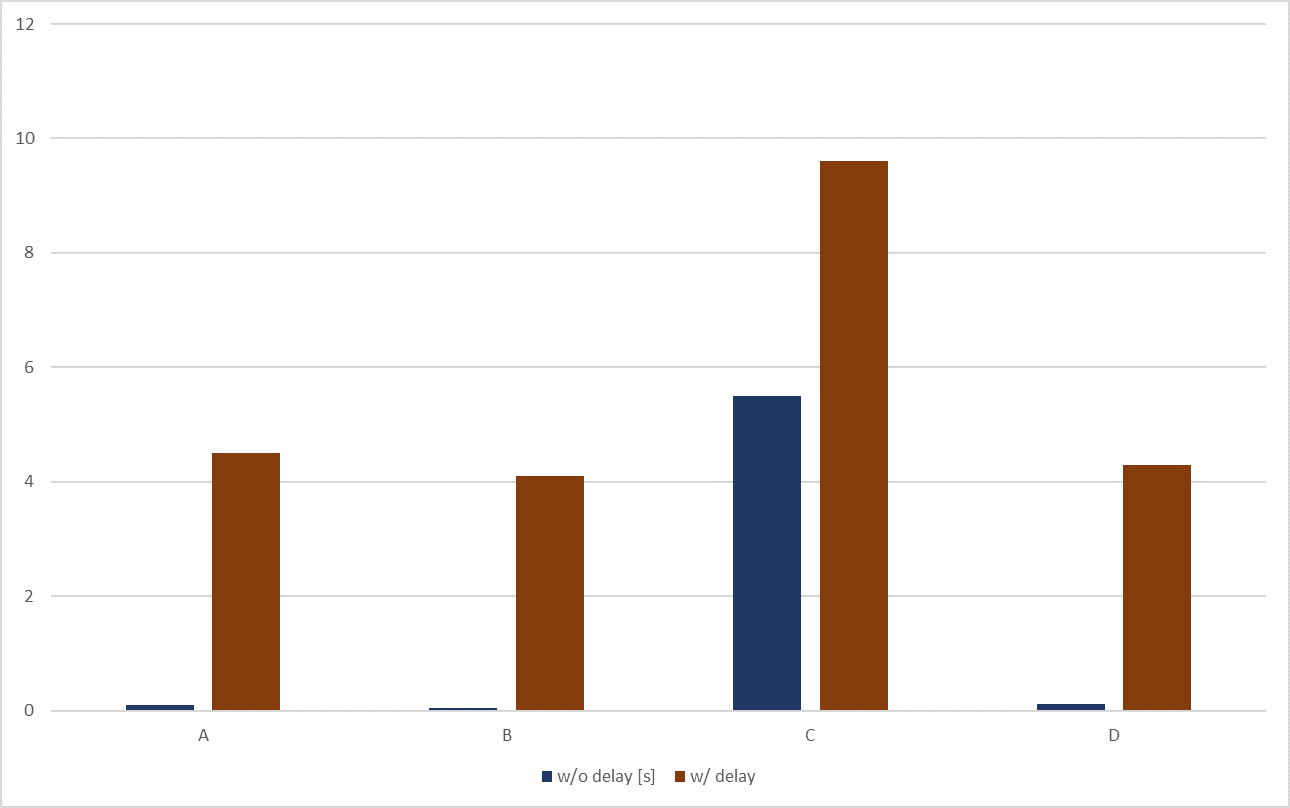
\includegraphics[width=\textwidth,height=\textheight,keepaspectratio]{results1.png}
    \caption{Comparision of scenarios and artificial delay introduced.}
    \label{fig:results}
  \end{center}
\end{figure}


This shows a clear impact of the artificial delay, since it's adds a constant 4s to the 100 requests.
Scenario \textit{E} is special and has to be interpreted.
In the case without an artificial delay, it's impact is \textless1\%, but sometimes more noticeable.
Contrary to this, running the server with an artificial delay between request elevates the time it takes to complete by up to 50\%.

\subsection{Multiprocessor tests}
Several test were made on clientLocal (4 logical cores) using the files created in the assignment without modifications and the provided \textit{rudy4.erl} \& \textit{test2.erl}.
Several combinations running an erlang shell with 1,2 \& 4 cores support were done. This is achieved by executing the shell with \textit{-smp enabled +S N} where \textit{N} is the desired amout of simultaneous processes being supported.
\\The observations made are clearly.
\textit{Test2.erl} is made to do several runs at the same time while in the server the function \textit{handlers/2} creates several processes for for listening to incoming connections.
Still, this didn't seem to make an impact, contrary to the influence of the amount of enabled multi processes given to the erlang shell.
As long as the amount is in the range of the amount of logical cores present, there's a proportional effect.

\begin{table}[h]
\centering
\begin{tabular}{lc}
Amount of processes enabled           & Time [ms]  \\\hline
1      &  2000\\\hline
2      & 1000\\\hline
4     & 500-550\\\hline
\end{tabular}
\caption{Relationship}
\label{tab:relations}
\end{table}

\section{Conclusions}

The problem gave some good ideas about how to implement a server to respond via HTTP instead of the normal messagin of Erlang. This gives a more universal approach since sockets and HTTP are in many, if not all progamming languages, present.


\end{document}
